\documentclass[journal,12pt,twocolumn]{IEEEtran}

\usepackage{setspace}
\usepackage{gensymb}

\singlespacing


\usepackage[cmex10]{amsmath}

\usepackage{amsthm}

\usepackage{mathrsfs}
\usepackage{txfonts}
\usepackage{stfloats}
\usepackage{bm}
\usepackage{cite}
\usepackage{cases}
\usepackage{subfig}

\usepackage{longtable}
\usepackage{multirow}

\usepackage{enumitem}
\usepackage{mathtools}
\usepackage{steinmetz}
\usepackage{tikz}
\usepackage{circuitikz}
\usepackage{verbatim}
\usepackage{tfrupee}
\usepackage[breaklinks=true]{hyperref}
\usepackage{graphicx}
\usepackage{tkz-euclide}
\usepackage{float}

\usetikzlibrary{calc,math}
\usepackage{listings}
    \usepackage{color}                                            %%
    \usepackage{array}                                            %%
    \usepackage{longtable}                                        %%
    \usepackage{calc}                                             %%
    \usepackage{multirow}                                         %%
    \usepackage{hhline}                                           %%
    \usepackage{ifthen}                                           %%
    \usepackage{lscape}     
\usepackage{multicol}
\usepackage{chngcntr}

\DeclareMathOperator*{\Res}{Res}

\renewcommand\thesection{\arabic{section}}
\renewcommand\thesubsection{\thesection.\arabic{subsection}}
\renewcommand\thesubsubsection{\thesubsection.\arabic{subsubsection}}

\renewcommand\thesectiondis{\arabic{section}}
\renewcommand\thesubsectiondis{\thesectiondis.\arabic{subsection}}
\renewcommand\thesubsubsectiondis{\thesubsectiondis.\arabic{subsubsection}}


\hyphenation{op-tical net-works semi-conduc-tor}
\def\inputGnumericTable{}                                 %%

\lstset{
%language=C,
frame=single, 
breaklines=true,
columns=fullflexible
}
\begin{document}
\newtheorem{theorem}{Theorem}[section]
\newtheorem{problem}{Problem}
\newtheorem{proposition}{Proposition}[section]
\newtheorem{lemma}{Lemma}[section]
\newtheorem{corollary}[theorem]{Corollary}
\newtheorem{example}{Example}[section]
\newtheorem{definition}[problem]{Definition}

\newcommand{\BEQA}{\begin{eqnarray}}
\newcommand{\EEQA}{\end{eqnarray}}
\newcommand{\define}{\stackrel{\triangle}{=}}
\bibliographystyle{IEEEtran}
\providecommand{\mbf}{\mathbf}
\providecommand{\pr}[1]{\ensuremath{\Pr\left(#1\right)}}
\providecommand{\qfunc}[1]{\ensuremath{Q\left(#1\right)}}
\providecommand{\sbrak}[1]{\ensuremath{{}\left[#1\right]}}
\providecommand{\lsbrak}[1]{\ensuremath{{}\left[#1\right.}}
\providecommand{\rsbrak}[1]{\ensuremath{{}\left.#1\right]}}
\providecommand{\brak}[1]{\ensuremath{\left(#1\right)}}
\providecommand{\lbrak}[1]{\ensuremath{\left(#1\right.}}
\providecommand{\rbrak}[1]{\ensuremath{\left.#1\right)}}
\providecommand{\cbrak}[1]{\ensuremath{\left\{#1\right\}}}
\providecommand{\lcbrak}[1]{\ensuremath{\left\{#1\right.}}
\providecommand{\rcbrak}[1]{\ensuremath{\left.#1\right\}}}
\theoremstyle{remark}
\newtheorem{rem}{Remark}
\newcommand{\sgn}{\mathop{\mathrm{sgn}}}
\providecommand{\abs}[1]{\left\vert#1\right\vert}
\providecommand{\res}[1]{\Res\displaylimits_{#1}} 
\providecommand{\norm}[1]{\left\lVert#1\right\rVert}
%\providecommand{\norm}[1]{\lVert#1\rVert}
\providecommand{\mtx}[1]{\mathbf{#1}}
\providecommand{\mean}[1]{E\left[ #1 \right]}
\providecommand{\fourier}{\overset{\mathcal{F}}{ \rightleftharpoons}}
%\providecommand{\hilbert}{\overset{\mathcal{H}}{ \rightleftharpoons}}
\providecommand{\system}{\overset{\mathcal{H}}{ \longleftrightarrow}}
	%\newcommand{\solution}[2]{\textbf{Solution:}{#1}}
\newcommand{\solution}{\noindent \textbf{Solution: }}
\newcommand{\cosec}{\,\text{cosec}\,}
\providecommand{\dec}[2]{\ensuremath{\overset{#1}{\underset{#2}{\gtrless}}}}
\newcommand{\myvec}[1]{\ensuremath{\begin{pmatrix}#1\end{pmatrix}}}
\newcommand{\mydet}[1]{\ensuremath{\begin{vmatrix}#1\end{vmatrix}}}
\numberwithin{equation}{subsection}
\makeatletter
\@addtoreset{figure}{problem}
\makeatother
\let\StandardTheFigure\thefigure
\let\vec\mathbf
\renewcommand{\thefigure}{\theproblem}
\def\putbox#1#2#3{\makebox[0in][l]{\makebox[#1][l]{}\raisebox{\baselineskip}[0in][0in]{\raisebox{#2}[0in][0in]{#3}}}}
     \def\rightbox#1{\makebox[0in][r]{#1}}
     \def\centbox#1{\makebox[0in]{#1}}
     \def\topbox#1{\raisebox{-\baselineskip}[0in][0in]{#1}}
     \def\midbox#1{\raisebox{-0.5\baselineskip}[0in][0in]{#1}}
\vspace{3cm}
\title{ASSIGNMENT 4}
\author{G.Rajanarsavva}
\maketitle
\newpage
\bigskip
\renewcommand{\thefigure}{\theenumi}
\renewcommand{\thetable}{\theenumi}
Download all python codes from 
\begin{lstlisting}
https://github.com/grajanarsavva/ASSIGNMENT4/tree/main/ASSIGNMENT4/CODES
\end{lstlisting}
%
and latex-tikz codes from 
%
\begin{lstlisting}
https://github.com/grajanarsavva/ASSIGNMENT4/tree/main/ASSIGNMENT4
\end{lstlisting}
%
\section{Question No 2.21}
Find the equation of plane passing through the points
a = \myvec{2 \\ 5 \\ -3} ; b = \myvec{-2 \\ -3 \\ 5} and c = \myvec{5 \\ 3 \\ -3} .
% 
\section{SOLUTION} 
The equation of plane is also given by (2.1.4.5).Following previous results in the matrix equation
\begin{enumerate}
\begin{align}
\myvec{2 & 5 & -3\\-2 & -3 & 5\\5 & 3 & -3} \vec{n} = \myvec{1\\1\\1}
\end{align}
% n^T\vec{x} = 1 
Row reducing the argumented matrix ,
\begin{align}
\myvec{2 & 5 & -3 & 1\\-2 & -3 & 5 & 1\\5 & 3 & -3 & 1}\\ 
\xleftrightarrow[R_3\leftarrow 2R_3-5R_1]{R_2\leftarrow \frac{R_2+R_1}{2}}\myvec{2 & 5 & -3 & 1\\0 & 1 & 1 & 1\\0 & -19 & 9 & -3}
\\
%\myvec{2 & 5 & -3 & 1\\0 & 1 & 1 & 1\\0 & -19 & 9 & -3}
\xleftrightarrow[R_3\leftarrow \frac{R_3+19R_2}{4}]{R_3\leftarrow R_1-5R_2}\myvec{2 & 0 & -8 & -4\\0 & 1 & 1 & 1\\0 & 0 & 7 & 4}
\\
%\myvec{2 & 0 & -8 & -4\\0 & 1 & 1 & 1\\0 & 0 & 7 & 4}
\xleftrightarrow[R_1\leftarrow \frac{7R_1+8R_2}{2}]{R_3\leftarrow 7R_2-R_3}\myvec{7& 0& 0 & 2\\0 & 7 & 0 & 3\\0 & 0  & 7 & 4}
%\myvec{7 & 0 & 0 & 2\\0 & 7 & 0 & 3\\0 & 0  & 7 & 4}
\end{align}
\begin{align}
\implies \vec{n} = \frac{1}{7}\myvec{2\\3\\4}
\end{align}
Thus,the equation of the plane passing through the given points is 
\begin{align}
\myvec{2 & 3 & 4}\vec{x} = 7  
\end{align}
Plot of the plane 
\numberwithin{figure}{section}
\begin{figure}[ht]
\centering
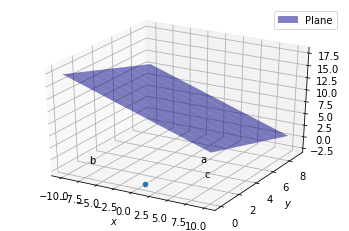
\includegraphics[width=\columnwidth]{Figure4.png}
\caption{Plot of the plane}
\label{Plot of the plane}
\end{figure}
\end{enumerate}
\end{document}